\documentclass[review]{elsarticle}

\usepackage[colorlinks]{hyperref}
\usepackage[colorinlistoftodos]{todonotes}
\usepackage{verbatim}
\usepackage[utf8]{inputenc}
\usepackage[T1]{fontenc}
\usepackage{adjustbox}
\usepackage{multirow}
\usepackage{longtable}
\usepackage{booktabs}
\usepackage{lineno,hyperref}
\usepackage{listings}
\modulolinenumbers[5]

\journal{colleagues for review}

%%%%%%%%%%%%%%%%%%%%%%%
%% Elsevier bibliography styles
%%%%%%%%%%%%%%%%%%%%%%%
%% To change the style, put a % in front of the second line of the current style and
%% remove the % from the second line of the style you would like to use.
%%%%%%%%%%%%%%%%%%%%%%%

%% Numbered
%\bibliographystyle{model1-num-names}

%% Numbered without titles
%\bibliographystyle{model1a-num-names}

%% Harvard 
%\bibliographystyle{model2-names.bst}\biboptions{authoryear}

%% Vancouver numbered
%\usepackage{numcompress}\bibliographystyle{model3-num-names}

%% Vancouver name/year
%\usepackage{numcompress}\bibliographystyle{model4-names}\biboptions{authoryear}

%% APA style
\bibliographystyle{model5-names}\biboptions{authoryear}

%% AMA style
%\usepackage{numcompress}\bibliographystyle{model6-num-names}

%% `Elsevier LaTeX' style
%\bibliographystyle{elsarticle-num}
%%%%%%%%%%%%%%%%%%%%%%%

\begin{document}

\begin{frontmatter}

%% Title, authors and addresses

\title{Shape difference or shape change? Inter-regional variation in Gahagan biface morphology}

%% use the tnoteref command within \title for footnotes;
%% use the tnotetext command for the associated footnote;
%% use the fnref command within \author or \address for footnotes;
%% use the fntext command for the associated footnote;
%% use the corref command within \author for corresponding author footnotes;
%% use the cortext command for the associated footnote;
%% use the ead command for the email address,
%% and the form \ead[url] for the home page:
%%
%% \title{Title\tnoteref{label1}}
%% \tnotetext[label1]{}
%% \author{Name\corref{cor1}\fnref{label2}}
%% \ead{email address}
%% \ead[url]{home page}
%% \fntext[label2]{}
%% \cortext[cor1]{}
%% \address{Address\fnref{label3}}
%% \fntext[label3]{}


%% use optional labels to link authors explicitly to addresses:
%% \author[label1,label2]{<author name>}
%% \address[label1]{<address>}
%% \address[label2]{<address>}
%% Group authors per affiliation:
\author{Robert Z. Selden, Jr.\textsuperscript{a,b,c*}, John E. Dockall\textsuperscript{d,e}, and Morgane Dubied\textsuperscript{f}}
\address[1]{Heritage Research Center, Stephen F. Austin State University, United States}
\address[2]{Cultural Heritage Department, Jean Monnet University, France}
\address[3]{ORCID ID \href{http://orcid.org/0000-0002-1789-8449}{0000-0002-1789-8449}}
\address[4]{Prewitt and Associates, Inc., United States}
\address[5]{ORCID ID \href{http://orcid.org/0000-0002-0940-7144}{0000-0002-0940-7144}}
\address[6]{UMR 6282, Laboratoire Biogéosciences, Université de Bourgogne, France}
\cortext[cor1]{Corresponding author, Robert Z. Selden, Jr. (zselden@sfasu.edu)}

\begin{abstract}
This investigation aggregates intact or reconstructed Gahagan bifaces from the Caddo and central Texas regions to test the hypothesis that Gahagan biface morphology differs between the two regions. The bifaces were scanned, then analysed using the tools of geometric morphometrics. Results provide a preview of the morphological differences that occur in Gahagan bifaces found at Caddo and central Texas sites. The size disparity represents an inversion of theoretical constructs that posit a decrease in tool size thought to articulate with an increase in distance from raw material source, as the bulk of the Caddo sample is thought to have been produced of Edwards chert from central Texas. One hypothesis (shape difference) posits that the contrasting morphologies may represent two discrete communities of practice; one (central Texas) where the bifaces were potentially utilised for more practical purposes, and the other (Caddo) where Gahagan bifaces were enlisted in burial and ritualistic activities. An alternative hypothesis (shape change) posits that Gahagan bifaces may have served multiple functions in Caddo society that differ in their deployment within and beyond the southern Caddo area.
\end{abstract}

\begin{keyword}
bifaces \sep NAGPRA \sep 3D \sep geometric morphometrics \sep museum studies
\end{keyword}

\end{frontmatter}

\linenumbers

\section*{}

\begin{quote}
The mathematical definition of a ``form'' has a quality of precision which was quite lacking in our earlier stage of mere description; it is expressed in few words, or in still briefer symbols, and these words or symbols are so pregnant with meaning that thought itself is economised \citep[720-721]{RN11532}.    
\end{quote}

This contribution follows a recent study of Gahagan biface morphology that enlisted the three largest samples from the Gahagan Mound (16RR1), George C. Davis (41CE19), and Mounds Plantation (16CD12) sites in the southern Caddo area (Figure 1) \citep{RN11783}. The results of that study indicated a significant difference in shape for Gahagan bifaces found at the Mounds Plantation site when compared with those found at the Gahagan Mound and George C. Davis sites \citep[Figure 7]{RN11783}. The test for morphological disparity indicated that the sample from Gahagan Mound occupied a significantly greater range of morphospace than the sample from Mounds Plantation, providing limited evidence for discussions of specialisation and diversity. Morphological integration was also significant, meaning those traits used to characterise Gahagan biface shape (blade and base) were found to vary in a coordinated manner. The results confirmed the supposition advanced by \cite{RN3684} that the assemblage of Gahagan bifaces from the George C. Davis site compares favourably with those reported from the Gahagan Mound site \citep{RN5274,RN2740}.

The Gahagan type was suggested by Clarence H. Webb at the Caddo Conference in 1970 \citep{RN3684}, and was intended as a replacement for what \cite{RN800} had previously called Copena knives based upon similarities in form, but not---according to \cite{RN3684}---technology, between specimens found at the George C. Davis site and those reported by \cite{RN11562} in Alabama. Gahagan bifaces are said to differ from Copena bifaces in technology, and were named for the finely-crafted bifaces found by \cite{RN2740} at Gahagan Mound \citep{RN3684}; however, a description of technological differences thought to occur between Gahagan and Copena bifaces was not provided. \citet[22]{RN4924} later advanced a technological description for the type. Like the Gahagan bifaces from the George C. Davis site, those from the Gahagan Mound and Mounds Plantation sites demonstrate a relatively high degree of intra-type morphological variation. Additional specimens have been added to the analysis from known Caddo sites (Doc Marks and Pelican), which are contrasted with those recovered from central Texas sites (Bastrop State Park and Doerge Collection), and include an unprovenienced collection from the Brazos Valley Museum of Natural History (BVMNH) (Figure ~\ref{fig:fig2}), provide those data needed to test whether Gahagan biface morphology in central Texas differs from those found at Caddo sites in east Texas. The Doerge Collection is a large private collection that was donated to the BVMNH, and includes the largest collection of Gahagan bifaces found outside of the southern Caddo area \citep[Table 5]{RN4924}. No site-specific details were provided to the museum related to context, association, or cultural affiliation; however, the museum was informed that the whole of the collection was from Brazos County, Texas. Another small collection of Gahagan bifaces are curated at BVMNH, are unprovenienced, and assumed to come from the central Texas region. The single specimen from Bastrop State Park was found on the surface at 41BP882 by Emmy Lyn Francell, and is curated at the Texas Parks and Wildlife Department.

\begin{figure}[htbp]\centering
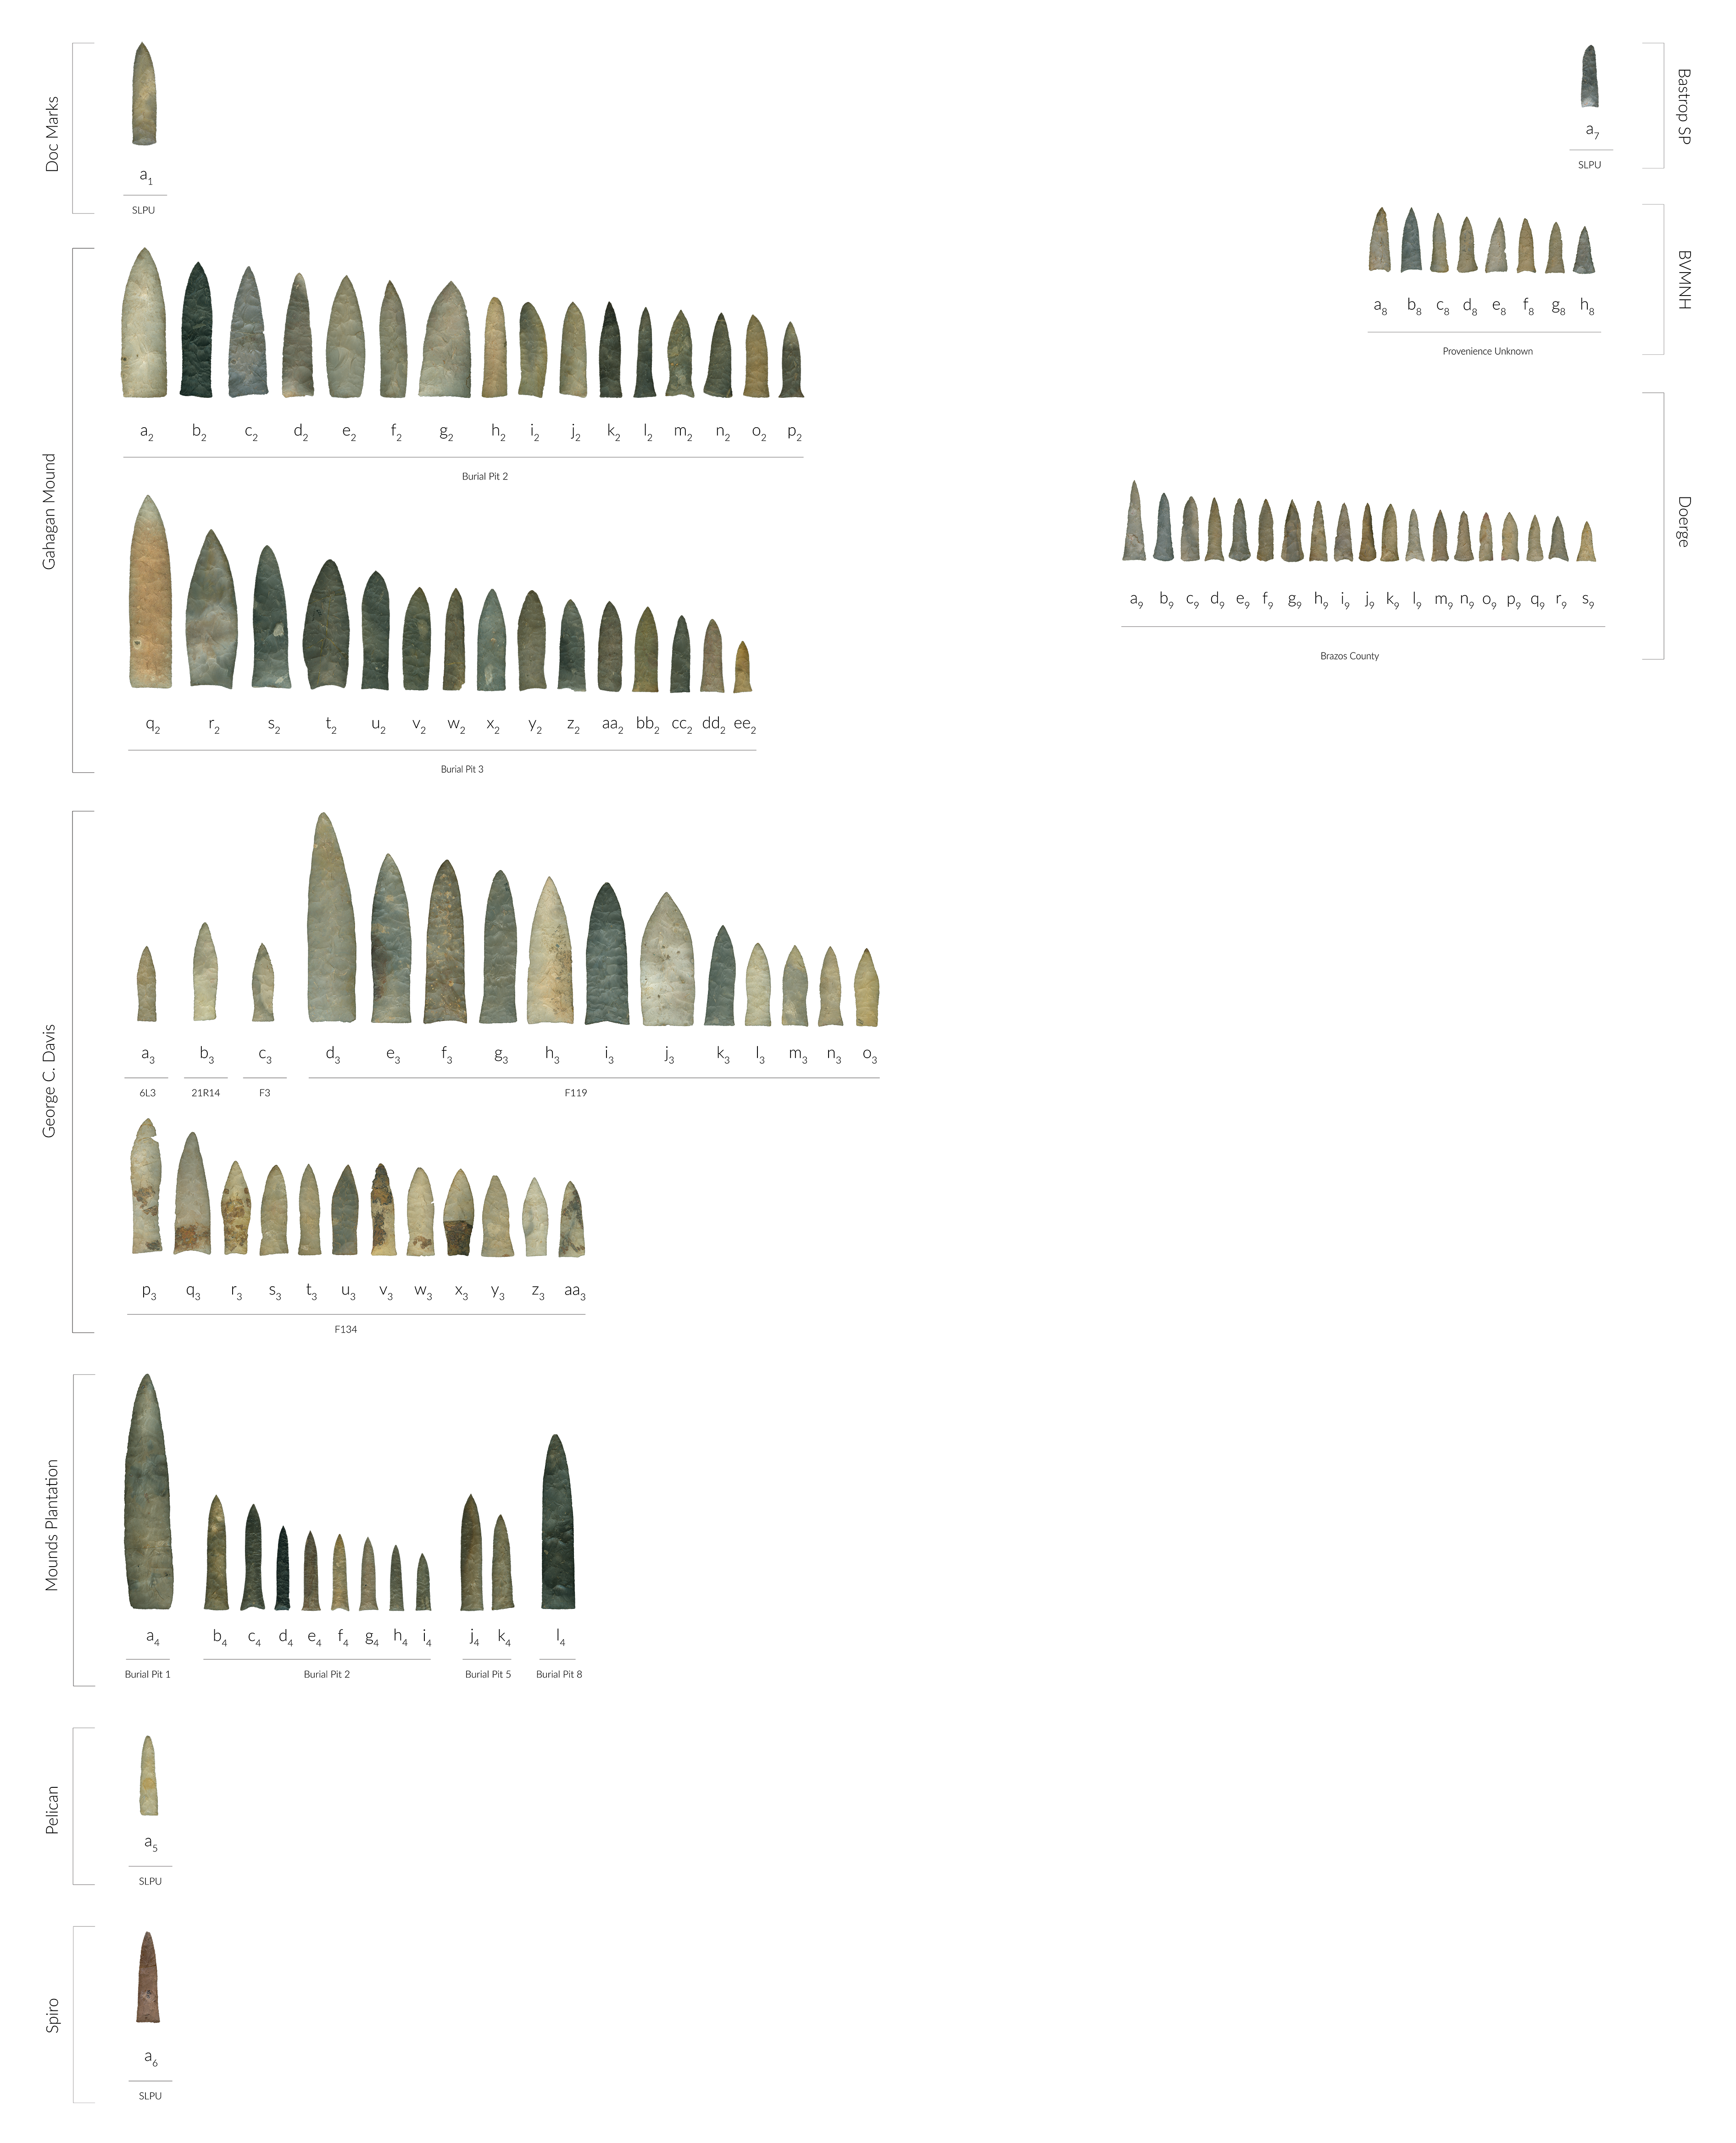
\includegraphics[width=\linewidth]{fig02}
\caption{Gahagan bifaces from known Caddo (left) and central Texas sites (right) organised by context and length; a1, no site-level provenience; a2, 569; b2, 543; c2, 551; d2, 541; e2, 546; f2, 544; g2, 545; h2, 489; i2, 532; j2, 548; k2, 550; l2, 533; m2, 549; n2, 547; o2, 490; p2, 542; q2, 593; r2, 666; s2, 605; t2, 622; u2, 606; v2, 609; w2, 623; x2, 608; y2, 607; z2, 662; aa2, 611; bb2, 610; cc2, 612; dd2, 613; ee2, 614; a3, ET221-993; b3, ET221-1260A; c3, ET221-1016; d3, 463-1; e3, 424-39; f3, 424-53; g3, 424-50; h3, 424-41; i3, 424-221; j3, 424-218; k3, 463-16; l3, 424-230; m3, 463-23; n3, 424-169; o3, 424-33; p3, 4078-8; q3, 4078-9; r3, 4078-11; s3, 4078-72; t3, 4078-45; u3, 4078-12; v3, 4078-13; w3, 4078-72; x3, 4078-14; y3, 4078-32; z3, 4078-22; aa3, 4078-14; a4, 3Ba90; b4, 3Bb6; c4, 3Bb1; d4, ThnBlk; e4, 3Bb7; f4, 3Bb3; g4, 3Bb4; h4, 3Bb8; i4, 3Bb5; j4, Case2LG; k4, Case2SM; l4, LGGray; a5, no site-level provenience; a6, no site-level provenience; a7 - h7, no provenience; a8 - s8, Brazos County, Texas. Bifaces w2, z2, and aa3 were not used in the analysis due to basal fractures, but are included here for visual comparative purposes. Additional information for each specimen, including the option to download the 2D images, can be found at \href{https://scholarworks.sfasu.edu/ita-gahaganbiface/}{https://scholarworks.sfasu.edu/ita-gahaganbiface/}.}
\label{fig:fig2}
\end{figure}

This effort represents the first formal comparison of Gahagan biface morphology across archaeological regions. Preliminary observations point to significant morphological differences between Gahagan bifaces recovered from Caddo and central Texas sites. Gahagan bifaces, a descriptive type including both morphological and chronological characteristics \citep{RN20847,RN4924,RN3684}, have long been leveraged as diagnostic markers of Formative and/or Early Caddo occupations. Should the morphology of Gahagan bifaces from central Texas be found to differ from those recovered from the southern Caddo area, additional theoretical explanations may be warranted. One possibility (shape difference) may be that two communities of practice existed for Gahagan bifaces. An alternative explanation (shape change) may be situational, demonstrating that Gahagan bifaces served multiple functions within Caddo society; one applied within the southern Caddo area, and another beyond. A third explanation is that both a shape difference and a shape change may be evidenced in Gahagan bifaces that may be further demarcated through an examination of context and chronology.

\subsection*{Context}

The flexuous blade shapes associated with Gahagan bifaces from Burial 1 at the Gahagan Mound site led to the initial interpretation that they were knives \citep[Figures 18-21]{RN2740}. A subsequent investigation at the Gahagan Mound site \citep{RN5274} classified the bifaces into two different biface types (neither of them Gahagan); one made of dull gray chert with a square base and a symmetrical or curved knife form, and the other made of semi-translucent flint with a curved base and more strongly curved sides. In Burial Pit 2 at Gahagan Mound \citep[Plate 21]{RN5274}, one Gahagan biface (Figure ~\ref{fig:fig2}, a2) \citep[Plate 27, No. 1, 3]{RN5274} was found near the left shoulder of an adult male (Skeleton 3), but most artefacts were recovered near the northwest margin of the burial pit, including the remaining Gahagan bifaces associated with that context. In Burial Pit 3 at Gahagan Mound \citep[Plate 23, 1]{RN5274}, one Gahagan biface was found near the left femur of Skeleton 1 (Figure ~\ref{fig:fig2}, r2) \citep[Plate 27, No. 1, 2]{RN5274}. Similar to Burial Pit 2, most of the artefacts from Burial Pit 3 were found along the northwest margin, including the remainder of Gahagan bifaces from that context \citep{RN5274}.

At the George C. Davis site, two Gahagan bifaces were found outside of mound or feature contexts (Figure ~\ref{fig:fig2}, a3 and b3), and their feature assignments (6L3 and 21R14) articulate with the excavation grid used by \cite{RN800}. Feature 3 is associated with a 27-foot diameter ring of 35 postholes located east of Mound A \citep[Figure 4]{RN800}. One Gahagan biface (Figure ~\ref{fig:fig2}, c3) was found in the outlining postholes \cite{RN800}.

Feature 134 is associated with a Stage I burial feature at the George C. Davis site that predates the construction of Mound C, and contained eight individuals \citep{RN808,RN5050}. One large (48 cm), well-thinned biface that \citet[22]{RN808} listed as a “Gahagan?” biface was found near the right leg of Skeleton 5.  \citet[Figure 19x]{RN3684} included this specimen---and one additional large specimen from Feature 119 \citep[Figure 19w]{RN3684}---in his Group 2 bifaces due to a lack of the fine pressure-flaked margins definitive of Group 1 (Gahagan) bifaces. Nine Gahagan bifaces from Feature 134 were recovered from Concentration 2; seven (Figure ~\ref{fig:fig2}, p3-r3, u3, v3, x3, and aa3) were found “about and under gray pigment,” and two others were found outside of the pigmented area (Figure ~\ref{fig:fig2}, s3, w3) \citep[21-23 and Figure 12]{RN808}. Organic residue can still be found on a selection of these Gahagan bifaces \citep[Figure 2]{RN11783}, which \citet[228]{RN3684} notes, “may be the remains of leather or bark sheaths or cane wrapping.” Three additional Gahagan bifaces (Figure ~\ref{fig:fig2}, t3, y3, and z3) were found in Concentration 3 \citep[21-22 and Figure 12]{RN808}.

Feature 119 \citep[Figure 13-18]{RN808} articulates with a Stage II burial feature at the George C. Davis site that can be traced from the surface of the second mound stage, and included offerings associated with two discrete layers \citep{RN808,RN5050,RN806}. The first layer offerings include Gahagan bifaces from Concentration 1 (Figure ~\ref{fig:fig2}, o3), Concentration 2 (Figure ~\ref{fig:fig2}, e3, g3, h3, and n3), and Concentration 3 (Figure ~\ref{fig:fig2}, f3, i3, j3, and l3). Second layer offerings include Gahagan bifaces associated with Concentration 1 (Figure ~\ref{fig:fig2}, d3), Concentration 3 (Figure ~\ref{fig:fig2}, m3), and Skeleton 1 (Figure ~\ref{fig:fig2}, k3). 

Burial Pit 2 at Mounds Plantation is the only context that contained a single individual, and \citet[97]{RN11561} noted that “fine edge retouch leaves the edges with almost no serration or irregularity, altogether the finest flint knapping that we have seen from a Caddoan site” (Figure ~\ref{fig:fig2}, b4-i4). The bifaces from Burial Pit 2 at Mounds Plantation were found in a bundle, but those from Burial Pit 5 articulate with the males of Groups 1 and 2 (Figure ~\ref{fig:fig2}, j4 and k4, respectively), and were found in a context parallel to the left forearm, pointed toward the hand \citep[Figure 5]{RN11561}. The biface from Burial Pit 8 at Mounds Plantation (Figure ~\ref{fig:fig2}, l4) was found in the same position on the left forearm; however, the largest biface (Burial Pit 1, Skeleton 1; see Figure ~\ref{fig:fig2}, a4) was found across the chest of that individual \citep{RN11561}.

McKinney posited that Gahagan bifaces may have been carried in a sheath attached to the left forearm \citep{RN11561}. Similarly, \citet{RN3684} noted that---at the George C. Davis site---edge modification was confined to traces of polish and smoothing along the widest blade segments and near the tip on burial specimens, was more pronounced on specimens from non-mound contexts, and possibly represented sheath wear. The polish that \citet{RN3684} discussed supports McKinney’s hypothesis \citep{RN11561}, where the tip and lateral edges of the biface may have become polished while being worn in a sheath on the left forearm with the tip pointed toward the hand.

\subsection*{Chronology}

\citet[Table 1]{RN4783} reported three AMS radiocarbon dates from Burial Pit 2 at the Gahagan Mound site. The first (UGA12296), from Deposit 3 in Burial Pit 2, was fragmented wood—possibly cypress—from a copper-covered wooden object that \citet[99, Plate 29, No. 2, Object 5]{RN5274} describe as a pendant in the shape of an animal claw \citep{RN4783}. The second (ISGS A0465), found adjacent to the head of Skeleton 3 (adult female) in Burial Pit 2, was unidentifiable fragmented wood that \citet[96, Plate 21 and 28, Nos. 2-3]{RN5274} describe as square ear ornaments of copper-coated cypress wood \citep{RN4783}. The third (ISGS A0466), from Deposit 2 in Burial Pit 2, was not described by \citet[96]{RN5274}, but \citet[62]{RN4783} describe it as a leather-covered copper object.

\citet[Table 1]{RN3714} reported two radiocarbon dates (Tx-913 and Tx-1206) from contexts that yielded Gahagan bifaces, which are associated with the special mortuary in Mound C at the George C. Davis site \citep[Table 5]{RN3714}. The date from Feature 119 (Tx-913) is associated with the green fill placed atop the Caddo remains in the Stage II burial in Mound C \citep{RN3714}. The date from Feature 134 (Tx-1206) provided an age that \citet{RN3714} believed to be inconsistent with the stratigraphic position of the sample, thus it is excluded from the chronological model. Neither of the legacy dates from the George C. Davis site account for isotopic fractionation.

\citet[72]{RN11561} reported three dates from two logs found in Burial Pit 5 at the Mounds Plantation site. Two of those (Tx-55 and M-1446), both from Log 1, were described by \citet[72]{RN11561} as coming “from the upper set of timbers, about 50 cm above the pit floor.” The third (Tx-56), from Log 6, was described by \citet[72]{RN11561} as coming from “Log 6…nearer the center of the pit and just above the pit floor.” None of these three legacy dates account for isotopic fractionation. \citet{RN11561} omit the Log 6 (Tx-56) date from further discussions of the site, thus it is omitted from the chronological model.

Six of the chronometric dates listed above were included in the chronological model for Caddo contexts where Gahagan bifaces have been found (Figure 3). The oxcAAR library (\href{https://github.com/ISAAKiel/oxcAAR}{https://github.com/ISAAKiel/oxcAAR}) was used to build the chronological model in R, which was executed using OxCal 4.3.2 \citep{RN5514,RN20716} and the IntCal13 calibration curve \citep{RN4406}. The chronological model demonstrates the modeled age range for contexts where a selection of those Gahagan bifaces used in this study were recovered \citep{RN20850}. All contexts were plotted as a single phase associated with the Gahagan biface type, and the two dates associated with Log 1 at Mounds Plantation (Tx-55 and M-1446) were combined using the R\_Combine function \citep{RN20850}. Sensitivity analyses demonstrated that agreement with the date from F119 at George C. Davis shifted only one or two percentage points in either direction throughout ten variable iterations, indicating that the model is stable. There are no known chronometric dates available for those Gahagan bifaces recovered from the central Texas contexts used in this study.

\begin{figure}[ht]\centering
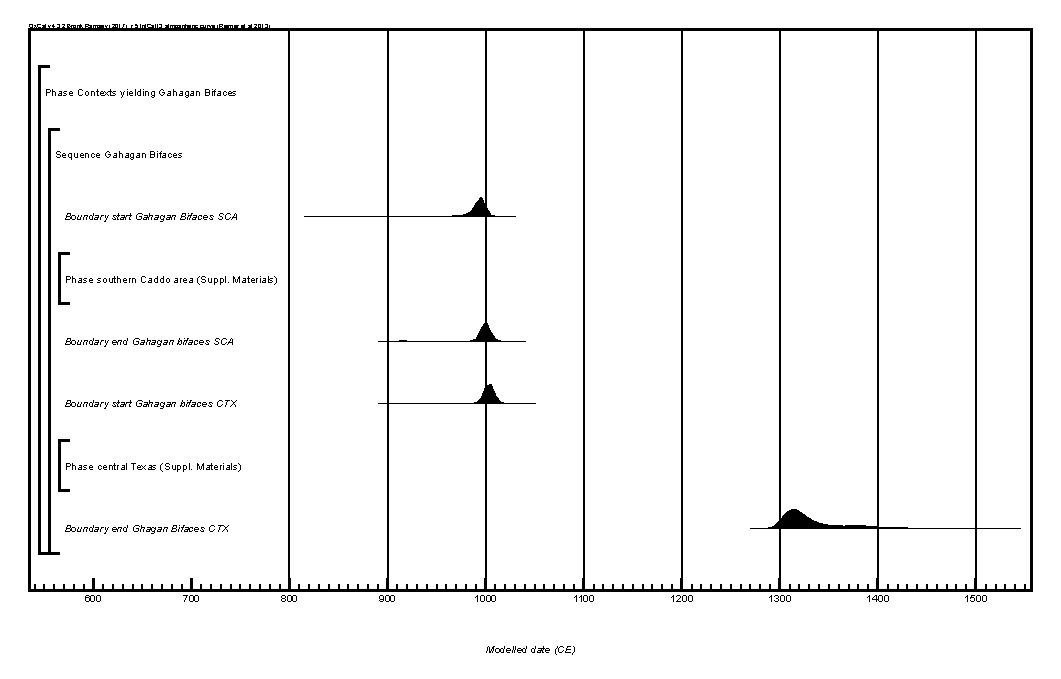
\includegraphics[width=\linewidth]{fig03}
\caption{Probability distributions for dates from contexts associated with Gahagan bifaces used in this study. Two distributions were plotted for each date or combination of dates; one represented by an outline that is the result of simple radiocarbon calibration, and the other in solid black, which articulates with the chronological model. The large square brackets down the left side of the diagram and the OxCal keywords define the model exactly. The oxcAAR script used to generate this figure is available at \href{https://github.com/seldenlab/14cgahagan/blob/master/gahaganb.md}{https://github.com/seldenlab/14cgahagan/blob/master/gahaganb.md}.}
\label{fig:fig3}
\end{figure}

\subsection*{Manufacture}

\citet{RN3684} discerned that all raw materials used in the manufacture of Gahagan bifaces found at the George C. Davis site were from non-local sources, which was a noteworthy revision to the initial interpretation by \citet{RN800}, in which the raw materials were considered to be of local origin. Further support for Shafer’s assertion is added in his discussion of the fragility of specimens coupled with the absence of failures in the extensive excavations at George C. Davis \citep{RN3684}. This observation aligns with findings from other locations \citep{RN1001}, where investigators demonstrated that Gahagan bifaces were manufactured with Woodford, Battiest, and Ogallala cherts, as well as cherts from the Kiamichi Mountains. \citet{RN3684} also noted the size and shape of Gahagan bifaces from the Davis site to be more uniform in Feature 134 compared with those from Feature 119, and that differences in the size of Gahagan bifaces from non-burial contexts were more striking than differences in shape.

\citet{RN3684} provides evidence for the presence of use-wear and fracture patterns on specimens from non-mound contexts at George C. Davis, suggesting that Gahagan bifaces from Caddo contexts may have functioned similarly to those used by hunter-gatherer groups. The occurrence of Gahagan bifaces in mound/burial and non-mound contexts at George C. Davis potentially indicates that they had secular and prestige/identity functions for Caddo peoples. In the analysis of debitage from George C. Davis, \citet{RN3684} argued that limited biface manufacture occurred at the site, but none of that debitage is directly attributable to Gahagan biface manufacture.

In addition to those Gahagan bifaces found at mound sites in the southern Caddo area, there is abundant evidence that similar bifaces were manufactured by contemporary hunter-gatherer groups in central and east-central Texas. Sites with evidence of manufacture and use can be found across a series of locations that fringe the eastern edge of the Balcones Escarpment \citep[Figure 5-3]{RN11568}. Each site is geographically situated on or within a zone of high-quality nodule and ledge cherts that may have served as source material. Gahagan bifaces found at these sites are represented by complete and incomplete specimens in varying stages of manufacture, use, maintenance, and discard. This indicates that bifaces were a commonly employed part of the overall lithic technology of central and east central Texas aboriginal groups, and likely used to perform a variety of common tasks.

A recent study tested the hypothesis that the manufacture of flat, thin bifaces—like Gahagan bifaces—would have yielded flatter bifacial thinning flakes that express low flake curvature \citep{RN11568}. The goal of that undertaking was to identify whether the flakes were distinctive enough on their own to warrant the assignment of potential Gahagan biface production locales, providing evidence for association of those production locales with the Prairie Caddo model \citep{RN4924} in the absence of diagnostic artefacts \citep{RN11568}. The results of that study demonstrated that bifacial thinning flake curvature was not sufficient as a marker of Gahagan biface production locales \citep{RN11568}.

In contrast to the Gahagan Mound, George C. Davis, and Mounds Plantation samples, there are currently no recorded instances of Gahagan bifaces from contexts in central Texas that might be interpreted as mortuary, religious, or ceremonial. Whether or not these bifaces served to denote individual status among hunter-gatherer groups is unknown, but they may have functioned as such during contact, exchange, or interaction between hunter-gatherers and Caddo groups to the east.

Production evidence is present at contemporary sites distributed on the eastern edge of the Balcones Escarpment. Sites like Urbankte (41CV26) and Penny Winkle (41BL22 and 41BL23), Iron Bridge (41BL47), Hoxie Bridge (41WM130), McDonald (41HI105), Loeve-Fox (41WM230), Grimes Houey (41CV17), J.B. White (41MM341) and locations on Fort Hood, have all yielded specimens representing manufacture, use and discard (Bond 1978, Gadus et al. 2006; Miller and Jelks 1952, Prewitt 1982, Shafer 2006, Shafer, Story, and Scurlock 1964). Shafer posited that these bifaces were manufactured through a mix of hard and soft hammer percussion, as well as indirect percussion using a punch \citep{RN4924,RN3684}. Flake scar patterns on many Gahagan bifaces support the inference that indirect percussion was used as a shaping and thinning technique. Isolated finds across Bell, Williamson, Milam, McLennan, and other counties in central Texas suggest that Gahagan bifaces were manufactured and used in these areas \citep{RN4924}.

\section*{Methods}

Each of the Gahagan bifaces was scanned with a Creaform GoSCAN 20 at a 0.3 mm resolution in VXelements. Scanner calibration was optimised prior to each scan with positioning targets required for increased accuracy and shutter speed reconfigured in each instance. A clipping plane was established to reduce the amount of superfluous data collected. Following data collection, the resolution of each mesh was increased to 0.1 mm, and the point cloud was transferred to VXmodel where the mesh was rendered following application of the \textit{clean mesh} function, used to remove isolated patches, self-intersections, spikes, small holes, singular vertices, creased edges, narrow triangles, outcropping triangles, narrow bridges, and non-manifold triangles prior to decimation and export as ASCII stl and ASCII ply. The stl functions as a 3D print-ready backup of the scan data, and the ply file was subsequently processed using the \textit{Rvcg} library in R 3.6.1 \citep{RN20849,R,RN20850}.

There is a residue adhering to seven of the Gahagan bifaces from the George C. Davis site that occurs at variable thicknesses \citep[Figure 2]{RN11783}. \citet[228]{RN3684} posits that this residue potentially represents the remains of a sheath. While an interesting aside, the residue does pose a problem for an analysis of 3D geometry. The initial research design (3D) was thus revisited, leading to a reconfiguration of the analysis as a 2D geometric morphometric study \citep{RN11783}, which enlisted a landmark configuration similar to that used by \citet[Figure 2]{RN1754}, \citet[Figure 2]{RN1736}, and \citet[Figure 1]{RN11731}. The residue does not occur on all of the George C. Davis specimens, and none of the Gahagan bifaces from the Mounds Plantation or Gahagan Mound sites include a similar residue on their surfaces, making it possible to compare a greater range of surface morphology between those samples. In reviewing the landmark configuration in advance of this study, the same basic constellation of landmarks was used; however, those landmarks were plotted directly on the meshes, providing a means of capitalising on shape variation introduced through the practice of beveling. This configuration of landmarks will be revised in subsequent iterations, where additional semilandmarks will be added to capture morphological attributes associated with Gahagan bifacial cross-sections, and other important morphological attributes. The evolution of this research program is focused not only upon aggregating additional specimens, but capitalising on the various morphological nuances and complexities included in those designs.

Two specimens in the George C. Davis sample (4078-8 and 4078-72), both from Feature 134, are missing small sections of their lateral edges (Figure ~\ref{fig:fig2} p3, w3). For the purpose of the GM analysis, these areas were modeled, and the surface of the mesh was extended to include the area of the missing piece in both instances \citep{RN20850}.

\subsection*{Alignment and Landmarks}

The \textit{auto3dgm} library \citep{RN20822} was used in in R 3.6.1 \citep{R} to align and compare the meshes leveraging principal alignments and minimising Procrustes distance between pseudolandmarks in advance of applying landmarks and semilandmarks. Subjective parameters used in the alignment included 250 initial points, and 1000 final points. The algorithm exported the aligned scans and a 3D image associated with the alignment and minimum spanning tree (Figure ~\ref{fig:fig4}). The image of the aligned bifaces produced by \textit{auto3dgm} was used as the basis for orienting the scans in 3D space throughout the process of applying landmarks and semilandmarks. This process aids in reducing investigator bias---although algorithmic bias is still introduced---through providing a method of selecting which face faces the investigator during the landmarking process..

\begin{figure}[ht]\centering
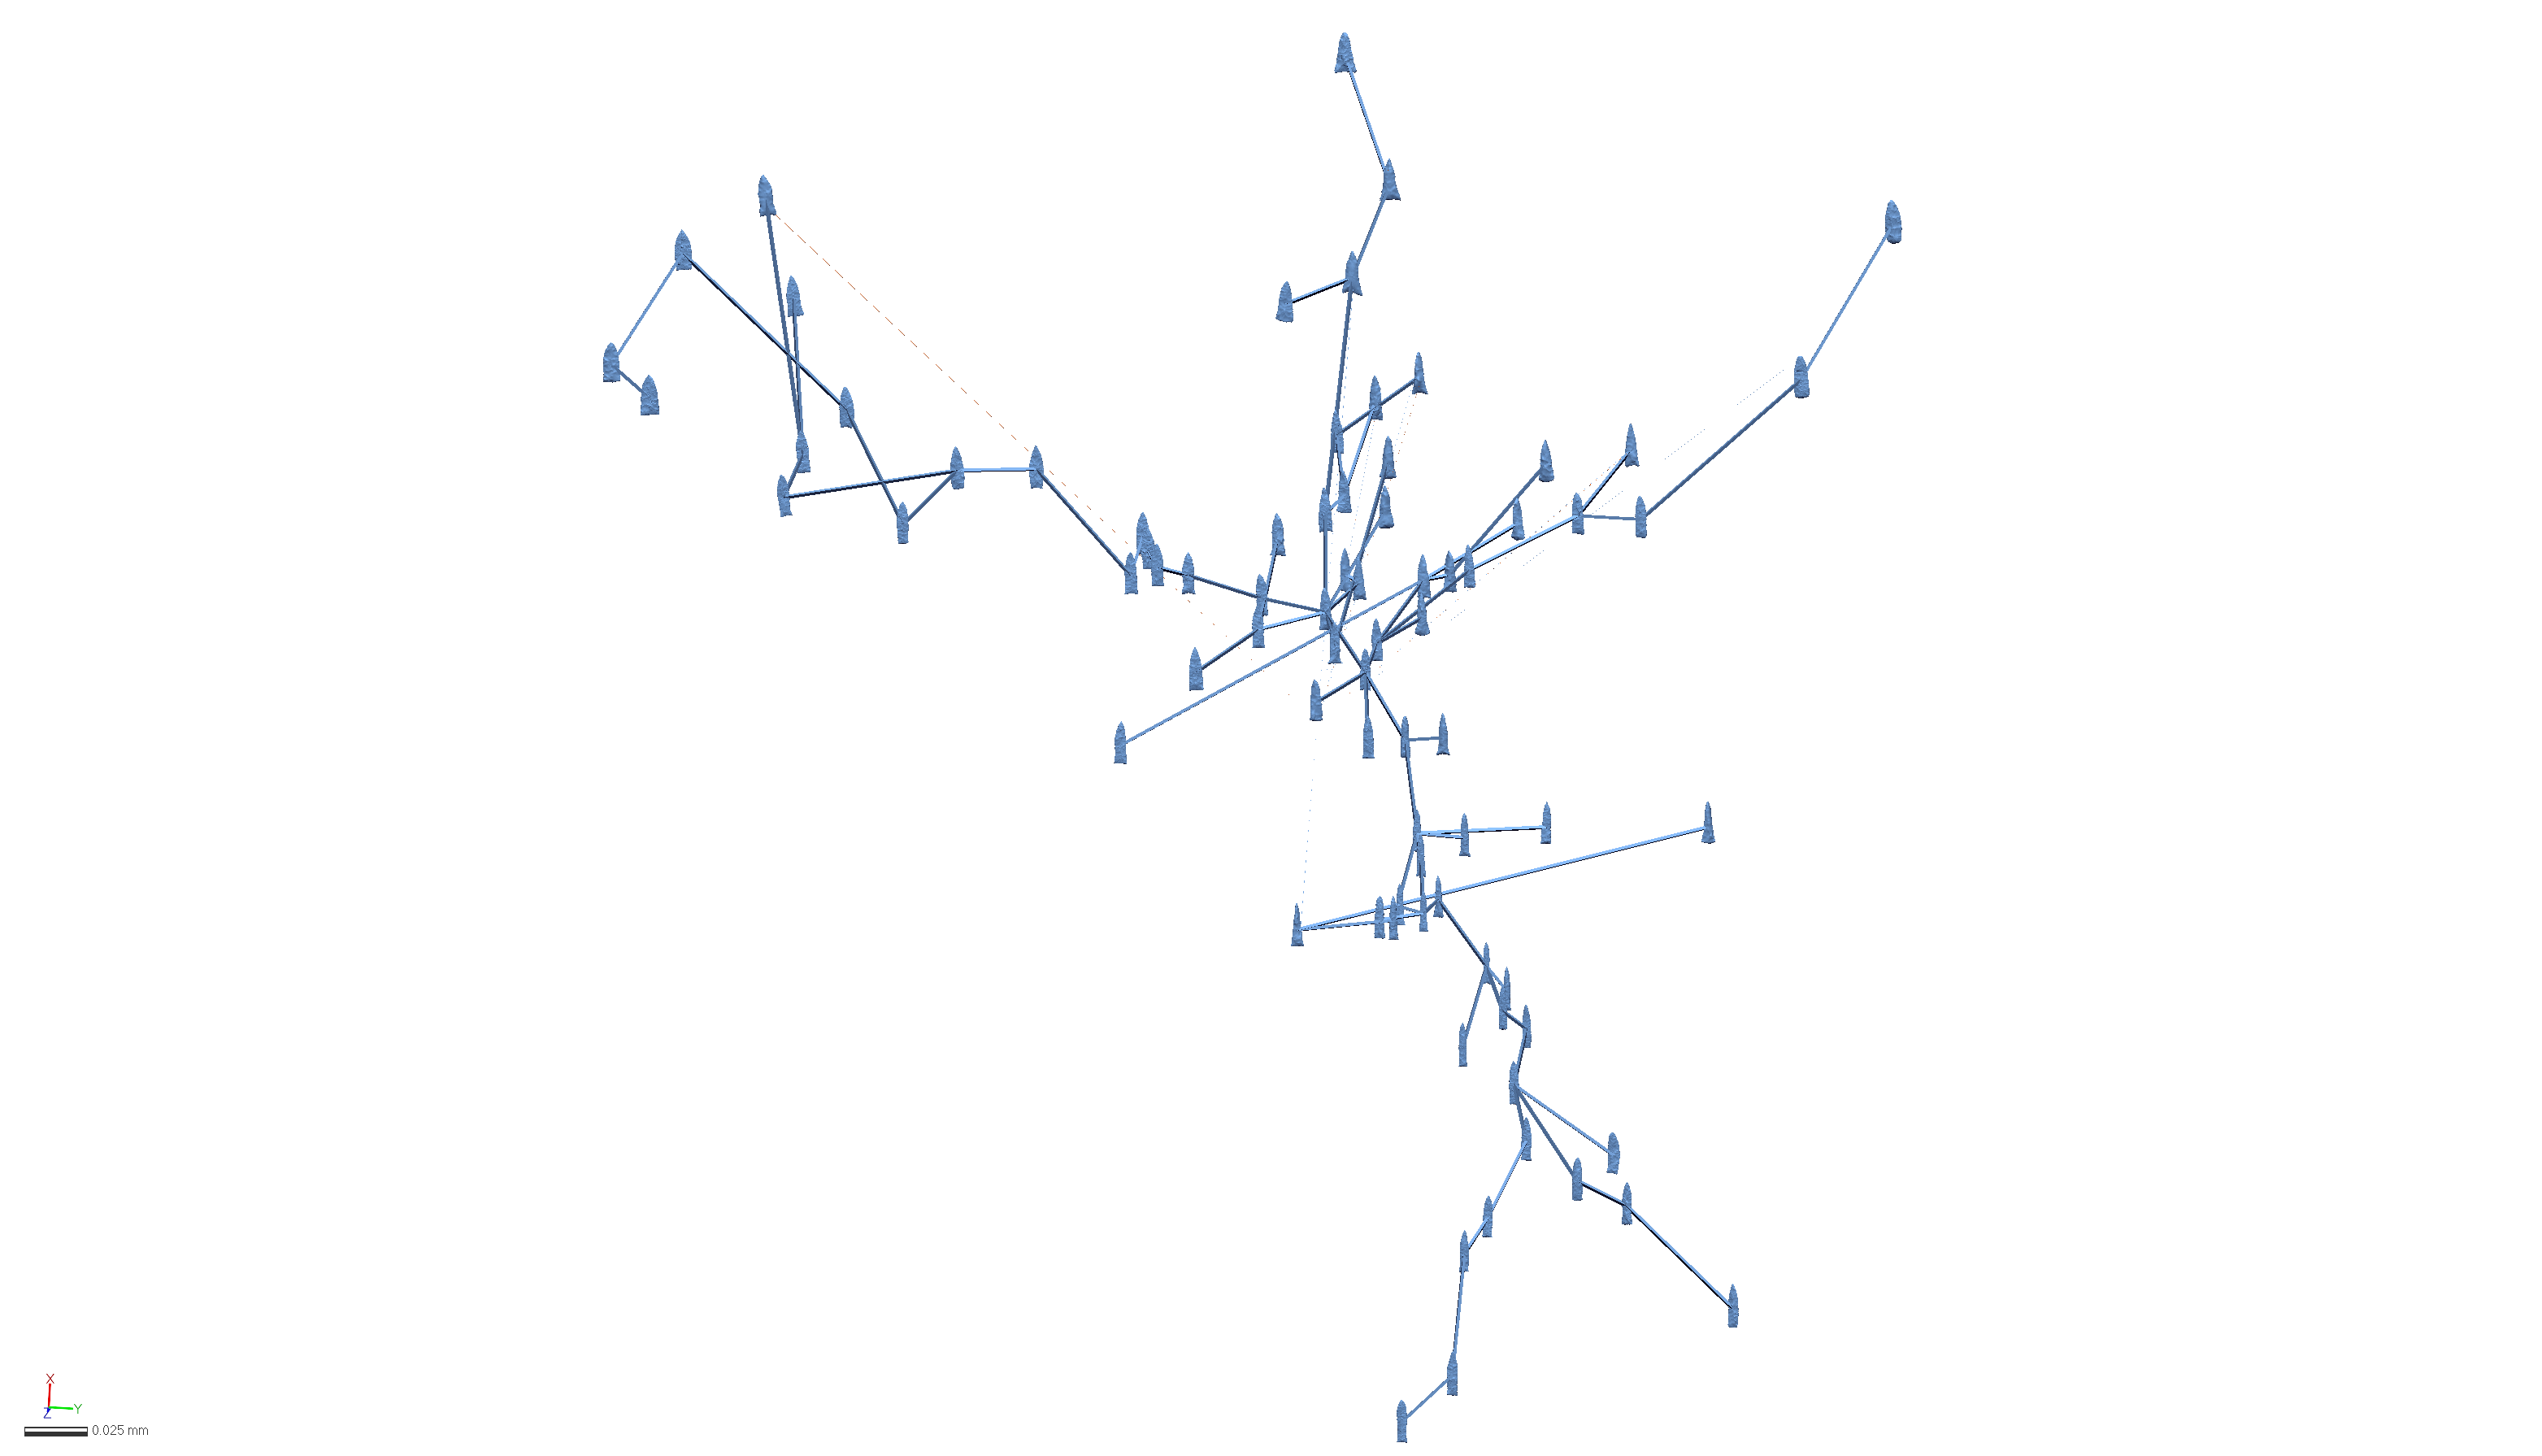
\includegraphics[width=\linewidth]{fig04}
\caption{Placeholder image. Figure caption will be added when final MST is rendered.}
\label{fig:fig4}
\end{figure}

The \textit{digit3DLand} library (\href{https://github.com/morphOptics/digit3DLand}{https://github.com/morphOptics/digit3DLand}) was used in R 3.6.1 \citep{R} to apply the landmarks and sliding semilandmarks (Table ~\ref{tab:Tbl1} and Figure ~\ref{fig:fig5}). The shift to a 3D analysis was made due to the amount of beveling that occurs in the sample of Gahagan bifaces. The same basic configuration of landmarks and semilandmarks used in the previous study \citep[Figure 3]{RN11783} was repurposed for this iteration; however, these landmarks and semilandmarks were placed directly on the mesh, providing a means of capitalising on the curvature that occurs along the lateral edges associated with beveling.

\begin{table}[tbh]\centering
\footnotesize
\caption{Landmarks used in the analysis. The position of the biface in 3D space was determined using the \textit{auto3dgm} alignment prior to applying the landmarks using \textit{digit3DLand}.}
\centering
\begin{tabular}{lcp{7.5cm}}
\toprule
Landmark & Location & Definition\\
\midrule
Point01 & Tip & Horizontal tangent\\
Point02 & Blade/Base & Point of highest curvature on right side\\
Point03 & Blade/Base & Point of highest curvature on left side\\
Point04 & CentreBase & Equidistant between Points 2 and 3\\
\bottomrule
\end{tabular}
\label{tab:Tbl1}
\end{table}

\begin{figure}[ht]\centering
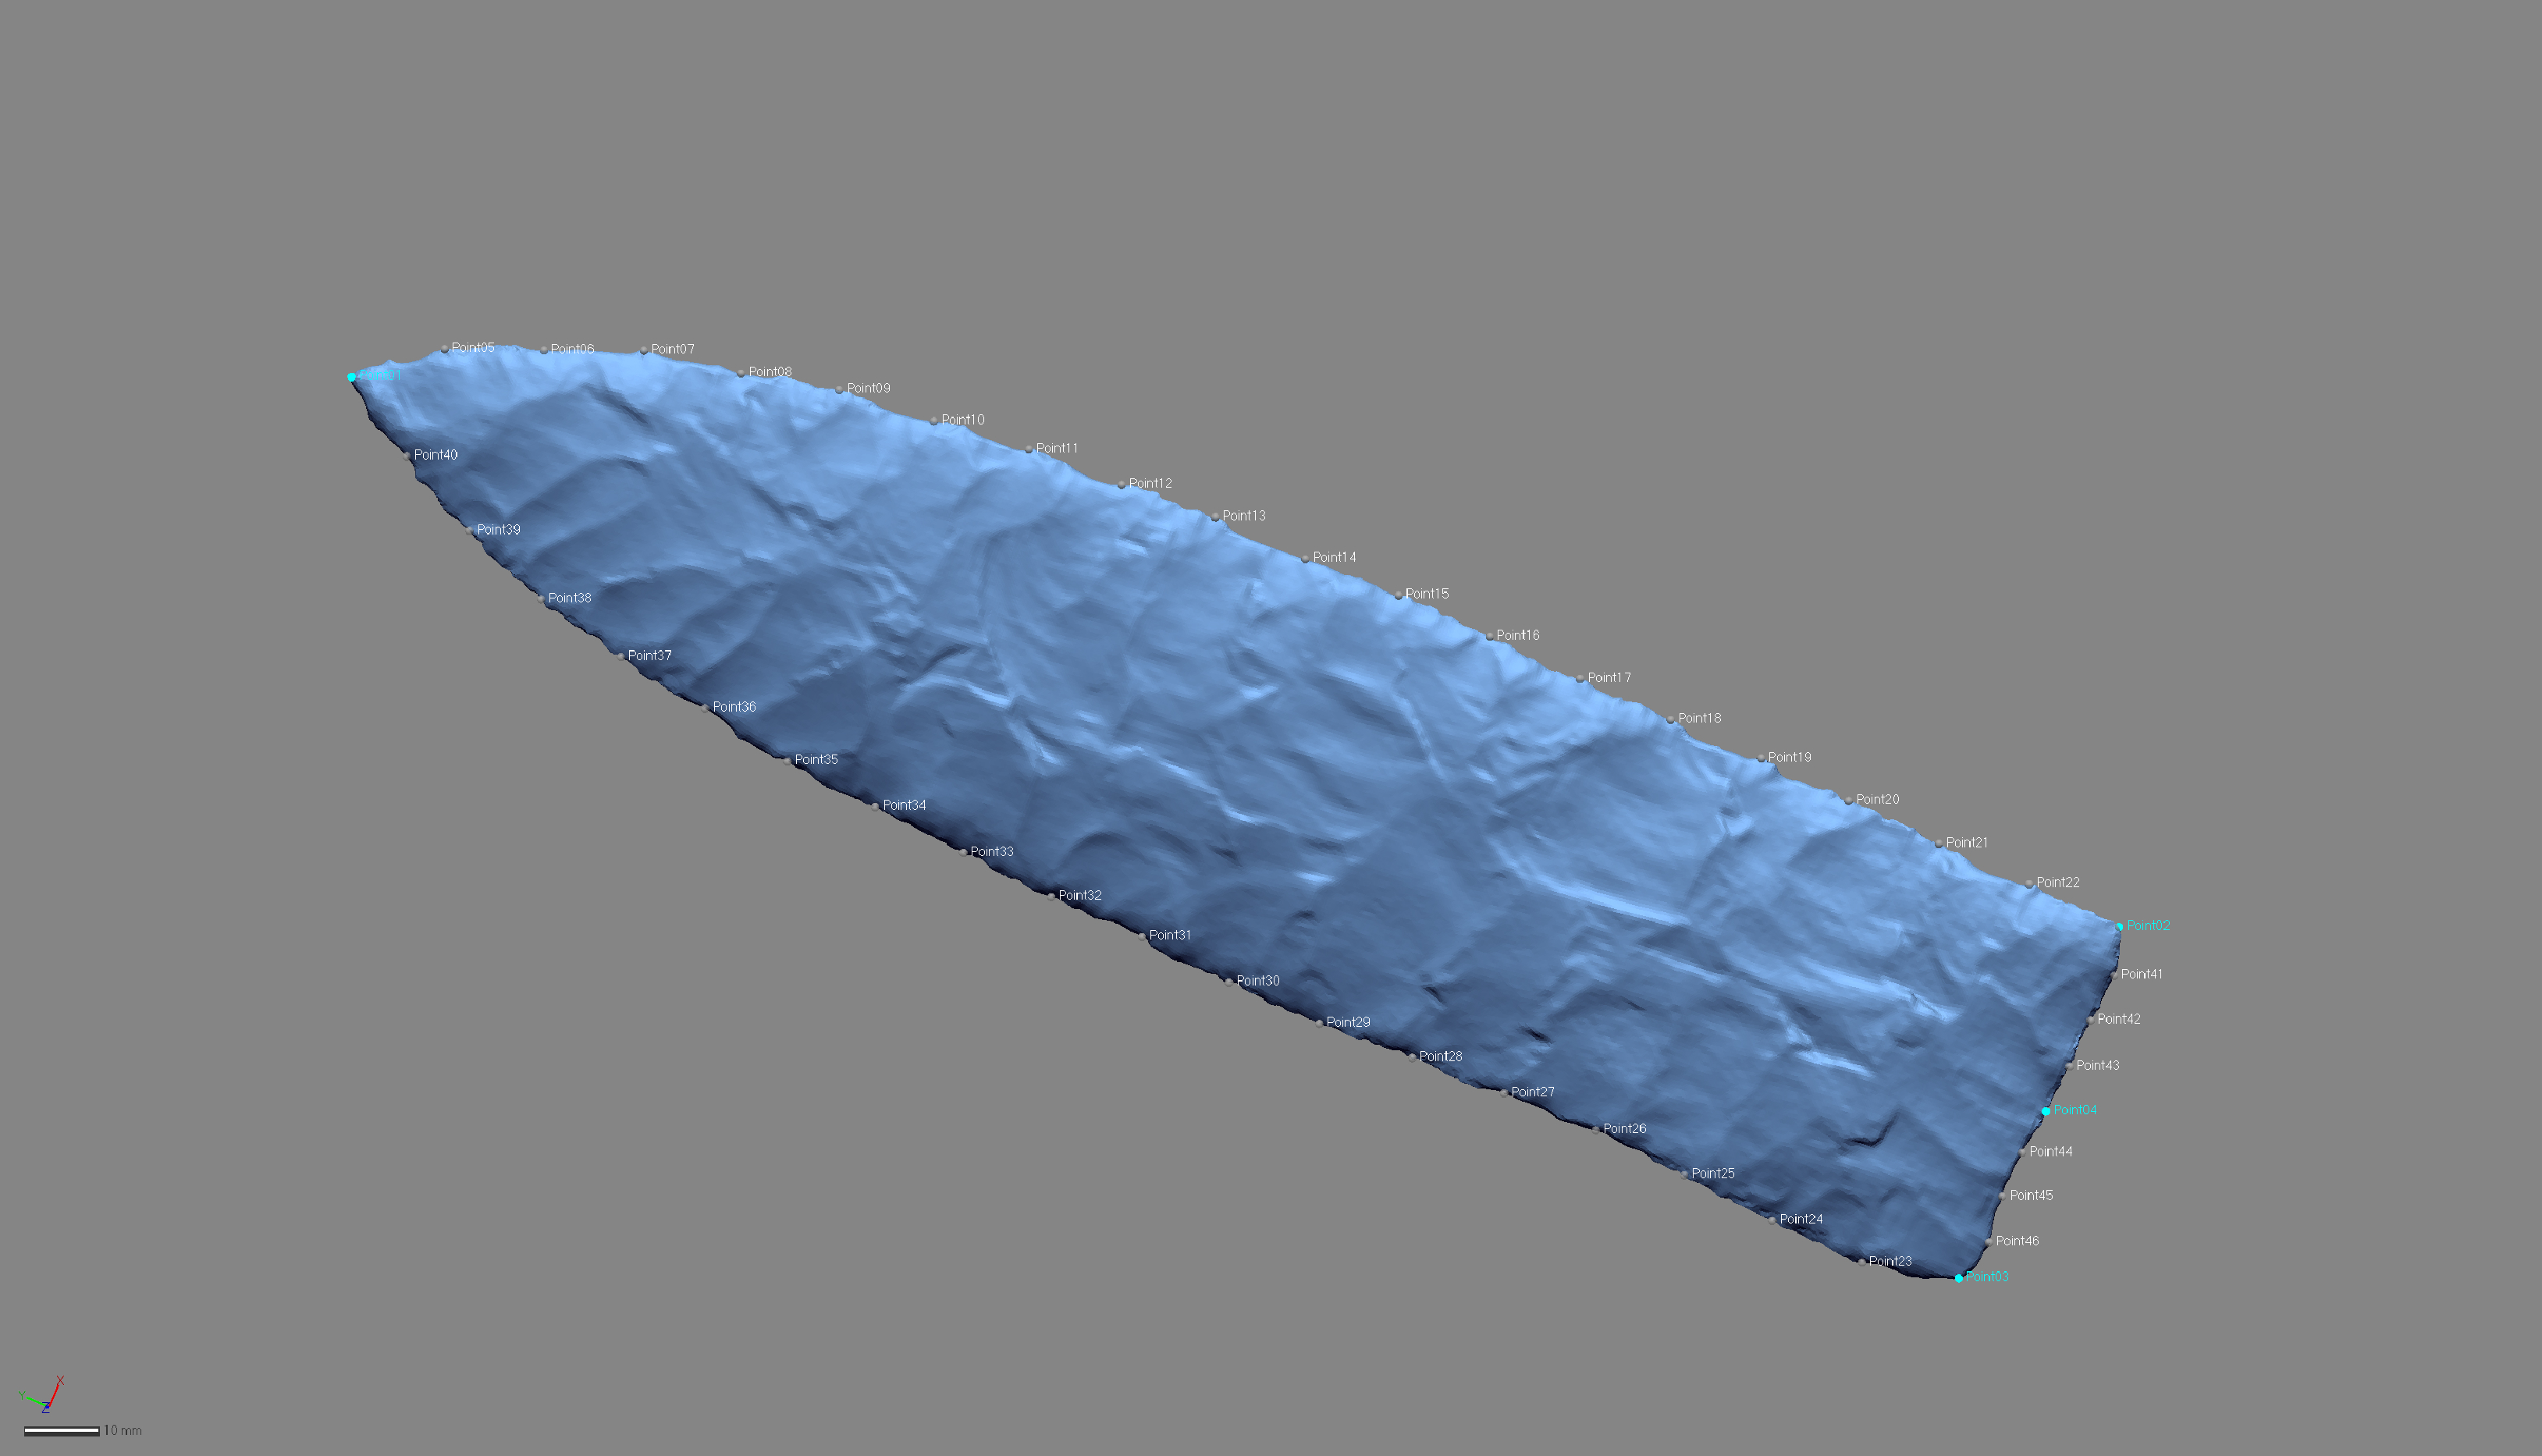
\includegraphics[width=\linewidth]{figlm}
\caption{Landmark (blue) and semilandmark (white) placement.}
\label{fig:fig5}
\end{figure}

\subsection*{Analysis}

Landmark data were aligned to a global coordinate system \citep{RN11622,RN11623,RN11563}, achieved through generalised Procrustes superimposition \citep{RN478} performed in R 3.6.1 \citep{R} using the \textit{geomorph} library v.3.1.2 \citep{RN11530,RN1774}. Procrustes superimposition translates, scales, and rotates the coordinate data to allow for comparisons among objects \citep{RN11564,RN478}. The \textit{geomorph} package uses a partial Procrustes superimposition that projects the aligned specimens into tangent space subsequent to alignment in preparation for the use of multivariate methods that assume linear space \citep{RN1646,RN11563}.

Principal components analysis \citep{RN1746} was used to visualise shape variation among the bifaces. The shape changes described by each principal axis are commonly visualised using thin-plate spline warping of a reference 3D mesh \citep{RN1731,RN479}. A residual randomisation permutation procedure (RRPP; n = 10,000 permutations) was used for all Procrustes ANOVAs \citep{RN1655,RN11775}, which has higher statistical power and a greater ability to identify patterns in the data should they be present \citep{RN1719}. To assess whether shape changes with size (allometry), and differs by group (region), Procrustes ANOVAs \citep{RN1749} were also run that enlist effect-sizes (z-scores) computed as standard deviates of the generated sampling distributions \citep{RN1756}. 

A Procrustes ANOVA and pairwise test was used to identify contexts where biface shapes differ, and enlists only those contexts where two or more specimens were recovered. The pairwise test is conceptually similar to trajectory analysis \citep{RN11573,RN1648,RN1776,RN1739} in that pairwise statistics are vector lengths between vectors, but differs since a factorial model is not explicitly needed to contrast vectors between point factor levels nested within group factor levels \citep{RN11530}. Procrustes variance was used to discriminate between groups and compare the amount of shape variation (morphological disparity) across regions \citep{RN11560}, estimated as the Procrustes variance using residuals of linear model fit \citep{RN11530}.

\section*{Results}

The mean consensus configuration and Procrustes residuals were calculated for each region by means of a generalised Procrustes analysis (GPA) \citep[Figure 3]{RN1720} (Figure ~\ref{fig:figGPA}). This initial view of these data demonstrates the mean shape and degree of variation that occurs in each region and across the whole sample. As an exploratory measure, GM methods---to include GPA---aid in clarifying shape differences associated with each population and in the production of novel \textit{a posteriori} hypotheses \citep{RN1720}.

\section*{Discussion}

\section*{Conclusion}

\section*{Acknowledgments}

We extend our gratitude to the Caddo Tribe of Oklahoma, the Williamson Museum at Northwestern State University, the Louisiana State Exhibit Museum, the Texas Archeological Research Laboratory at The University of Texas at Austin, the Brazos Valley Museum of Natural History, and the Texas Parks and Wildlife Department for the requisite permissions and access needed to generate the 3D scans of the Gahagan bifaces. Thanks to Harry J. Shafer, Jeffrey S. Girard, Hiram F. (Pete) Gregory, Julian A. Sitters, Timothy K. Perttula, and David K. Thulman for their comments on a draft of this manuscript. Thanks also to Dean C. Adams, Michael L. Collyer, Emma Sherratt, Lauren Butaric, and Kersten Bergstrom for their constructive criticisms, comments, and suggestions throughout the development of this research design, and to the editors and anonymous reviewers for their comments and constructive criticisms, which further improved the manuscript.

Components of this analytical work flow were developed and funded by a Preservation Technology and Training grant (P14AP00138) to RZS from the National Center for Preservation Technology and Training, and funding to scan the Gahagan bifaces at the Williamson Museum at Northwestern State University, Louisiana State Exhibit Museum, and Texas Archeological Research Laboratory at The University of Texas at Austin was provided to RZS by the Heritage Research Center at Stephen F. Austin State University.

\bibliography{mybibfile}

\end{document}